% 编译: latexmk -xelatex paper_mzm_zh.tex
\documentclass[journal]{IEEEtran}
\usepackage{amsmath,amssymb,amsthm}
\usepackage{bm}
\usepackage{graphicx}
\usepackage{stfloats}   % 允许 figure*/table* 落在双栏页面的底部，增加跨栏浮动体的排版余地
\usepackage{booktabs}
\usepackage{array}
\usepackage{cite}
\usepackage{algorithm}
\usepackage{algpseudocode}
\floatname{algorithm}{算法}
\renewcommand{\algorithmicrequire}{\textbf{输入:}}
\renewcommand{\algorithmicensure}{\textbf{输出:}}
\usepackage{fontspec}
% Load by filename (kpathsea-searched in texmf-dist) for cross-platform builds
% (Windows/macOS/Linux) -- avoids OS font-name lookup and hardcoded paths.
\setmainfont{texgyretermes-regular.otf}[
  BoldFont=texgyretermes-bold.otf,
  ItalicFont=texgyretermes-italic.otf,
  BoldItalicFont=texgyretermes-bolditalic.otf]
\makeatletter
\edef\@tmp{\noexpand\DeclareFontFamilySubstitution{TU}{ptm}{\rmdefault}}\@tmp
\makeatother
\usepackage{xeCJK}
% On macOS, Songti produces a Poppler-readable CID embedding; fall back to the
% TeX-distributed Fandol files on systems without Songti.  The prior unconditional
% Fandol embedding rendered as blank CJK glyphs in Poppler despite being embedded.
\IfFontExistsTF{Songti SC}{
  \setCJKmainfont[AutoFakeBold=2.5,AutoFakeSlant=0.18]{Songti SC}
  \setCJKsansfont[AutoFakeBold=2.5]{Heiti SC}
  \setCJKmonofont{Songti SC}
}{
  \setCJKmainfont[
    BoldFont={FandolSong-Bold.otf},
    ItalicFont={FandolKai-Regular.otf}
  ]{FandolSong-Regular.otf}
  \setCJKsansfont[
    BoldFont={FandolHei-Bold.otf}
  ]{FandolHei-Regular.otf}
  \setCJKmonofont{FandolFang-Regular.otf}
}
% IEEE journal 惯例：段首缩进由 IEEEtran 提供，首段不缩进（去掉 indentfirst）。
% 中文正文用两个汉字宽度的段首缩进：10pt 正文下一个汉字宽 10pt=1em，故 2em=2 汉字，
% 比 IEEE 默认 1em 更符合中文排版。
\setlength{\parindent}{2em}
\usepackage[colorlinks=false,pdfborder={0 0 0}]{hyperref}

\renewcommand{\abstractname}{摘\quad 要}
\renewcommand{\IEEEkeywordsname}{关键词}
\renewcommand{\figurename}{图}
\renewcommand{\tablename}{表}
\renewcommand{\appendixname}{附录}
\renewcommand{\refname}{参考文献}

\theoremstyle{plain}
\newtheorem{theorem}{定理}
\newtheorem{lemma}{引理}
\newtheorem{proposition}{命题}
\theoremstyle{remark}
\newtheorem{remark}{注}
\renewcommand{\proofname}{证明}

\newcommand{\zv}{\mathbf{z}}
\newcommand{\uv}{\mathbf{u}}
\newcommand{\bv}{\mathbf{b}}
\newcommand{\nv}{\mathbf{n}}
\newcommand{\tv}{\mathbf{t}}
\newcommand{\vv}{\mathbf{v}}
\newcommand{\phiv}{\bm{\varphi}}
\newcommand{\Lc}{\mathcal{L}}
\newcommand{\atan}{\operatorname{atan2}}
\newcommand{\T}{\mathsf{T}}

\begin{document}

\title{基于精确仿射模型的MZM任意点偏压控制}

\author{第一作者，第二作者%
\thanks{作者单位：西安电子科技大学综合业务网理论及关键技术国家重点实验室，西安~710071（通信作者电子邮箱：author@xidian.edu.cn）。}}

\markboth{基于精确仿射模型的~MZM 任意点偏压控制}%
{作者~\MakeLowercase{\textit{等}}：基于精确仿射模型的~MZM 任意点偏压控制}

\maketitle

\begin{abstract}
马赫--曾德尔调制器（MZM）的任意点偏压控制要求在全周期内获得无死区、无分支歧义的相位反馈，而单谐波或谐波比值易受灵敏度零点和通道失配影响。本文建立线性接收--解调链下的精确仿射模型：在单余弦功率传递和测量窗内参数冻结条件下，一次与二次谐波观测是偏置相位单位圆的仿射像，增益失配、参考相位误差、导频同步电串扰和偏置无关的有限消光比统一进入通道矩阵与观测平移向量。基于该模型，通过全周期扫描辨识仿射参数并固定相位规范，闭式反演恢复偏置相位，进而以同一积分控制律锁定任意目标点。数值实验验证了模型的数值精确闭合、全周期反演和目标点无关的闭环增益。真实硬件在~16 个全周期目标点的静态相位标签评价中，二维仿射方案的跨目标均方根（root-mean-square, RMS）相位误差为~246~mrad；本文以该量表征任意点静态控制精度，H1 幅值匹配基线的对应误差为~1241~mrad。结果表明，精确仿射建模为~MZM 任意点偏压提供了可辨识、可标定且覆盖全周期的控制坐标。
\end{abstract}

\begin{IEEEkeywords}
马赫--曾德尔调制器，偏压控制，导频，仿射辨识，椭圆拟合，微波光子学。
\end{IEEEkeywords}

\IEEEpeerreviewmaketitle
\setlength{\emergencystretch}{2em}

\section{引言}
% 注：IEEEtran 的 \IEEEPARstart 首字下沉是为拉丁字母设计的，套用汉字（FandolSong）
% 会把汉字挤出下沉框、破坏首句字序，故此处按普通段首处理（中文期刊惯例）。
铌酸锂（LiNbO$_3$）、磷化铟（InP）以及薄膜铌酸锂马赫--曾德尔调制器（MZM）的工作点会随温度、电荷积累和光折变效应缓慢漂移~\cite{salvestrini2011,chen2011,wang2018,wang2022}。小幅低频导频（dither）能够在不中断业务信号的条件下持续观测这种漂移：探测光电流的一次谐波（H1）在最大/最小透射点（峰/谷点）附近过零，二次谐波（H2）在正交点附近过零，由此形成闭环误差信号。面向开关键控（OOK）、同相/正交（IQ）调制器和偏振复用发射机的特殊点锁定及其多环扩展已经形成成熟的实现路线~\cite{cho2006,sotoodeh2011,kawakami2012,fu2013,li2017}。

微波光子移相器与矢量调制器~\cite{yao2009,capmany2007}、单边带（SSB）权重控制~\cite{izutsu1981}、模拟光计算~\cite{shen2017} 和啁啾管理还要求偏置稳定在传递曲线的连续设定点上。现有任意点方法包括单~MZM 的预标定谐波比值~\cite{wang2010}、平均功率导数或局部差分~\cite{tao2014,yuan2019}、面向具体链路的模型控制~\cite{teng2023}，以及~IQ 调制器中的专用抖动序列与相关检测~\cite{li2018,peng2025}。模型优化已用于单~MZM 的峰/谷点和正交点控制~\cite{svarny2022,weller2025}；近年来的研究中出现了以直流、H1 和导频相关乘积构造多维特征，通过神经网络与粒子群搜索实现任意点控制~\cite{hu2026dla2c}。这些方法分别利用标定比例、局部斜率、专用激励或在线优化建立偏置状态与观测特征之间的对应关系。

连续设定点控制的核心是从全周期（一个~$2\pi$ 偏置相位周期）中恢复偏置相位，同时把接收链的增益、偏置和通道混合与相位本身分离。单个光滑周期标量不可能在全周期上单射，并在临界点失去局部灵敏度；多维观测则需要进一步确定未知通道作用下的可辨识条件、分支方向和绝对相位基准。本文研究线性接收--解调链中的这一通道可辨识问题，并给出从二维谐波观测恢复全周期相位的精确条件。

本文证明，偏置相位与导频时间波形在余弦传递函数中可以精确分离；在测量窗内参数冻结时，任意线性接收--解调链输出的二维谐波观测必为偏置相位单位圆的仿射像。增益失配、参考相位误差、导频同步串扰和偏置无关的有限消光比只改变椭圆的位置、尺度和方向。满秩观测保证椭圆可逆；椭圆分解剩余的~$O(2)$ 规范包含反射与旋转歧义，扫描方向固定反射，直流相位锚点固定旋转和相位原点。在标定参数的有效期内，闭式反演给出全周期相位。该几何与位移干涉测量中的~Heydemann 校正~\cite{heydemann1981,fitzgibbon1999} 相通，本文进一步建立了偏压域中的绝对相位规范和闭环设定点对应关系。主要贡献如下：

\begin{enumerate}
\item \emph{精确观测结构与统一解释}。建立适用于任意周期导频波形和线性接收--解调链的精确仿射定理，给出通道矩阵、观测平移与随机噪声的闭式表达，并将特殊点锁定、H1 幅值匹配和谐波比值归结为二维观测的不同低维读出。
\item \emph{全周期辨识与闭式控制}。证明满秩观测与唯一规范固定构成全周期相位可辨识的充要条件，将标定分解为椭圆几何辨识、反射定向和绝对相位规范固定，并由此得到目标点无关的相位反演与积分控制律。
\item \emph{任意点控制与硬件验证}。数值实验验证数值精确闭合、全周期反演和目标点无关的闭环增益；真实硬件在~16 个全周期目标点取得~246~mrad 的跨目标静态相位~RMS，H1 幅值匹配基线为~1241~mrad。样本外相位反演、静态重复采集与逐射频（RF）状态重新标定进一步检验标定泛化、采集重复性和静态载荷下的可重标定性。
\end{enumerate}

第~\ref{sec:model} 节回顾信号模型与传统锁定；第~\ref{sec:affine}--\ref{sec:noise} 节建立精确仿射理论；第~\ref{sec:algo} 节给出标定与运行流程；第~\ref{sec:numerics} 节报告数值验证；第~\ref{sec:exp} 节给出平台实测；第~\ref{sec:discussion} 节讨论适用边界与推广方向。

\section{信号模型与传统导频锁定}
\label{sec:model}

\subsection{模型与解调泛函}
考虑推挽式单驱~MZM，臂间功率分配比为~$r$，
\begin{equation}
P_{\mathrm{out}}(t)=\tfrac{P_0}{2}\bigl[1+\eta\cos\varphi(t)\bigr],\quad
\eta=\tfrac{2\sqrt r}{1+r}\le 1,
\label{eq:mzm}
\end{equation}
其中~$P_0$ 为输入光功率，$\eta$ 为由臂间功率分配决定的条纹可见度。偏置相位~$\varphi_b=\pi V_b/V_\pi+\varphi_0$，其中~$V_b$、$V_\pi$、$\varphi_0$ 分别为偏压、半波电压和零偏相位；导频~$\xi(t)=m\sin\omega t$ 的角频率为~$\omega$，电压幅值为~$V_d$，相位调制深度为~$m=\pi V_d/V_\pi$，且~$\varphi(t)=\varphi_b+\xi(t)$。光电流分解为~$i(t)=\mathcal{R}P_{\mathrm{out}}(t)+i_x(t)+i_n(t)$，其中~$\mathcal{R}$ 为探测器响应度，$i_x$ 收集与导频\emph{相干}的确定性电学串扰，$i_n$ 为随机噪声过程。锁相解调建模为线性泛函
\begin{equation}
\Lc_1[f]\!\triangleq\!\overline{2f(t)\sin(\omega t{+}\theta_1)},\quad
\Lc_2[f]\!\triangleq\!\overline{2f(t)\cos(2\omega t{+}\theta_2)},
\label{eq:lockin}
\end{equation}
上横线表示低通时间平均，$\theta_1,\theta_2$ 为参考相位误差（含链路群延迟）。配以电增益~$G_1,G_2$，观测量定义为~$Y\triangleq G_1\Lc_1[i]$、$X\triangleq G_2\Lc_2[i]$。下文称~$\omega$ 通道（$Y$）为~H1、$2\omega$ 通道（$X$）为~H2。偏置相位~$\varphi_b$ 受温度等因素影响而缓慢漂移。解调带宽远高于漂移，平均窗远短于漂移时间尺度，故窗内~$\varphi_b$ 可视为常数。下列各式在每个控制周期取当前~$\varphi_b$ 值成立。

有记忆的稳定线性接收链可与锁相运算复合为等效泛函~$\Lc_j$。以下结论要求每个测量窗开始前链路已沉降，且窗内~$\varphi_b$ 近似不变。

理想光生电流项~$i_{\rm ph}=\mathcal{R}P_{\rm out}$ 的~Jacobi--Anger 展开为
\begin{equation*}
\begin{aligned}
i_{\rm ph}(t)
={}&\frac{\mathcal{R} P_0}{2}
\bigl[1+\eta J_0(m)\cos\varphi_b\bigr]\\
&+\eta\mathcal{R} P_0\cos\varphi_b
\sum_{k=1}^{\infty}J_{2k}(m)\cos(2k\omega t)\\
&-\eta\mathcal{R} P_0\sin\varphi_b
\sum_{k=0}^{\infty}J_{2k+1}(m)\sin[(2k{+}1)\omega t].
\end{aligned}
\end{equation*}
其中~$J_n$ 为第一类~$n$ 阶贝塞尔函数。偶次谐波和直流可变项携带~$\cos\varphi_b$，奇次谐波携带~$\sin\varphi_b$。当~$J_0(m),J_1(m),J_2(m)\neq0$ 时，直流分量提供规范基准，H1/H2 构成二维相位观测，并分别给出峰/谷点与正交点的传统锁定误差。理想极限（$\theta_i{=}0$、正弦~$\xi$、$i_x{=}0$）下，
\begin{equation}
Y=-\eta\kappa_1\sin\varphi_b,\quad X=\eta\kappa_2\cos\varphi_b,\quad
\kappa_n\triangleq G_n\mathcal{R} P_0 J_n(m),
\label{eq:ideal}
\end{equation}
其中~$\kappa_1,\kappa_2$ 即导频文献中熟知的谐波斜率系数。
定义单位圆特征向量
$\uv(\varphi_b)\triangleq(\cos\varphi_b,\sin\varphi_b)^{\T}\in\mathbb{S}^1$；其两个坐标分别承载偶次与奇次谐波的偏置相位信息。

\subsection{特殊点锁定及其静差}
\label{sec:conventional}
正交点锁定驱动~$X\to 0$。其局部增益~$|\mathrm{d}X/\mathrm{d}\varphi_b|=\eta\kappa_2|\sin\varphi_b|$ 在~$\pi/2$ 处取极大，两个正交点由~$\operatorname{sgn}Y$ 判别，过零点对共模功率波动一阶免疫。峰/谷点锁定驱动~$Y\to0$，增益~$\eta\kappa_1$，两点由~$\operatorname{sgn}X$ 判别。为统一表示接收链失配，记~$A=[A_{ij}]$ 为二维通道矩阵、$\bv=(b_X,b_Y)^{\T}$ 为观测平移向量，其完整表达在第~\ref{sec:affine} 节给出。分别在四个特殊点线性化锁定条件，得到
\begin{equation}
\begin{aligned}
\Delta\varphi_{\mathrm Q}^{(\pi/2)}&=\frac{A_{12}+b_X}{A_{11}},&
\Delta\varphi_{\mathrm Q}^{(3\pi/2)}&=\frac{A_{12}-b_X}{A_{11}},\\
\Delta\varphi_{\mathrm N}^{(0)}&=-\frac{A_{21}+b_Y}{A_{22}},&
\Delta\varphi_{\mathrm N}^{(\pi)}&=\frac{b_Y-A_{21}}{A_{22}}.
\end{aligned}
\label{eq:staticQ}
\end{equation}
上标标明展开点，不同半周期分支的偏置项符号不同。文献中报道的残余偏置误差由此统一写成非对角或偏置元素与对角斜率之比的形式。

每种特殊点方案都只读取~$\uv(\varphi_b)=(\cos\varphi_b,\sin\varphi_b)^{\T}$ 的\emph{一个}坐标，且只工作在该坐标的过零点邻域。在过零点处，局部斜率取极大，误差量过零使增益标定相消，另一坐标恰可充当符号判别量。一旦离开过零点，这三项便利同时失效。

\subsection{任意点控制的传统方案}
\emph{幅值匹配}：取~$e=Y-Y^\ast$，$Y^\ast=-\kappa_1^{\mathrm{nom}}\sin\varphi^\ast$ 由标称参数计算。其局部增益~$\propto\eta\kappa_1|\cos\varphi^\ast|$ 在正交点附近消失，形成死区。$Y$ 在~$\varphi\leftrightarrow\pi-\varphi$ 下不变，存在分支歧义。标称增益失配还会被死区因子放大为静差：
\begin{equation}
\Delta\varphi_{\mathrm{AM}}
=-\frac{A_{21}\cos\varphi^\ast+(A_{22}{+}\kappa_1^{\mathrm{nom}})
\sin\varphi^\ast+b_Y}{A_{22}\cos\varphi^\ast-A_{21}\sin\varphi^\ast}.
\label{eq:staticAM}
\end{equation}
\emph{谐波比值法}：$X/Y=-(\kappa_2/\kappa_1)\cot\varphi_b$ 消去了公共功率标量，但隐含假设~$A$ 为对角阵且~$\bv=0$。偏置项会破坏余切律，$Y\!\to\!0$ 邻域噪声按~$1/Y^2$ 放大，双象限歧义也仍然存在。一次除法只能消去一个公共标量，而真实失配是六参数的仿射群作用。

\begin{proposition}[拓扑障碍]
\label{prop:rolle}
由单个标量谐波特征~$g(\varphi_b)$ 构造的任何误差函数都是光滑的~$2\pi$ 周期函数，故每个周期内必有临界点~$g'(\varphi^\dagger)=0$（Rolle 定理），该处环路增益消失；且~$g$ 在一个周期上不可能单射。与之相对，$\varphi_b\mapsto\uv(\varphi_b)$ 是浸入~$\mathbb{S}^1\!\to\!\mathbb{R}^2$，满足~$\|\uv'\|\equiv 1$ 且在~$[0,2\pi)$ 上单射。
\end{proposition}

因此，对无记忆的瞬时静态读出而言，二维化是消除死区与歧义的最小代价。但物理系统给出的不是~$\uv$，而是它的一个未知形变像。下一节证明该形变只能是仿射的。

\section{精确仿射定理}
\label{sec:affine}

\begin{lemma}[相位因子分解]
\label{lem:fact}
对任意波形~$\xi(t)$，恒等式
$\cos(\varphi_b+\xi(t))=\cos\varphi_b\cos\xi(t)-\sin\varphi_b\sin\xi(t)$
精确成立：偏置相位与时间依赖完全因子化。导频波形决定线性映射，偏置相位决定单位圆上的位置。
\end{lemma}

\begin{theorem}[精确仿射性]
\label{th:affine}
设~$\xi(t)$ 为任意周期导频波形（不必正弦、不必小信号），接收为任意线性链路加线性解调泛函~$\Lc_1,\Lc_2$。记二维锁相观测为~$\zv\triangleq(X,Y)^{\T}$，则存在通道矩阵~$A\in\mathbb{R}^{2\times2}$、观测平移向量~$\bv\in\mathbb{R}^2$ 和随机噪声~$\nv\in\mathbb{R}^2$，使
\begin{equation}
\boxed{\;\zv=A\,\uv(\varphi_b)+\bv+\nv\;}
\label{eq:affine}
\end{equation}
精确成立，且
\begin{align}
A&=\frac{\eta\mathcal{R} P_0}{2}
\begin{pmatrix}
G_2\Lc_2[\cos\xi] & -G_2\Lc_2[\sin\xi]\\
G_1\Lc_1[\cos\xi] & -G_1\Lc_1[\sin\xi]
\end{pmatrix},\nonumber\\
 d_j&\triangleq\frac{\mathcal{R} P_0}{2}\Lc_j[1]+\Lc_j[i_x],\qquad j\in\{1,2\},\nonumber\\
\bv&=\begin{pmatrix}G_2d_2+O_X\\G_1d_1+O_Y\end{pmatrix},\quad
\nv=\begin{pmatrix}G_2\Lc_2[i_n]\\ G_1\Lc_1[i_n]\end{pmatrix},
\label{eq:entries}
\end{align}
其中~$O_X,O_Y$ 为混频器直流失调。
\end{theorem}
\begin{proof}
将引理~\ref{lem:fact} 代入
$i=\tfrac{\mathcal{R} P_0}{2}[1+\eta\cos(\varphi_b+\xi)]+i_x+i_n$，
利用~$\Lc_{1,2}$ 的线性逐项收集即得；光功率常数项经任意线性泛函产生的确定性输出统一进入~$\bv$。对式~\eqref{eq:lockin} 的完整周期正交锁相，$\Lc_{1,2}[1]=0$，式~\eqref{eq:entries} 相应退化为仅含串扰与混频器失调的常见形式。
\end{proof}

该结构的几何意义见图~\ref{fig:affine}(a)(b)：含失配的观测轨迹是单位圆~$\mathbb{S}^1$ 的仿射像。当且仅当~$\operatorname{rank}A=2$（等价于最小奇异值~$\sigma_{\min}(A)>0$）时，该像为非退化椭圆，仿射逆~$A^{-1}(\zv-\bv)$ 才能把观测唯一回拉至单位圆。秩亏链路只保留一个标量投影，不能支持全周期无歧义反演。$\Lc_1,\Lc_2$ 是线性泛函，只能对信号作叠加，无法混入乘积或高次项。引理~\ref{lem:fact} 已把偏置相位与导频波形分开，因此线性链输出只能是~$\cos\varphi_b$ 与~$\sin\varphi_b$ 的仿射组合。任何超出仿射的项（如~$\cos 2\varphi_b$）都需要非线性运算，故被线性性排除。

\begin{proposition}[全周期可辨识的充要条件]
\label{prop:ident}
设无噪全周期扫描覆盖~$\mathbb{S}^1$，接收--解调参数在扫描期间不变。由无序轨迹和单次观测唯一确定~$\varphi_b\bmod 2\pi$，当且仅当：(i)~$\operatorname{rank}A=2$；(ii)~辅助信息唯一固定椭圆分解的~$O(2)$ 规范，其中~$O(2)$ 为二维正交群。
\end{proposition}
\begin{proof}
若~$A$ 满秩，则其线性作用保持单位圆参数的单射性；规范固定后，$A^{-1}(\zv-\bv)=\uv(\varphi_b)$，故~$\atan$ 唯一给出模~$2\pi$ 相位。反之，若~$A$ 秩亏，观测至多为单位圆的一个标量投影，连续周期映射必有重复值；若规范未固定，则任意~$R\in O(2)$ 均产生同一轨迹，而对应相位相差未知旋转或反射。因此任一条件缺失都不能唯一辨识全周期相位。
\end{proof}

线性非理想因素统一通过~$A$ 和~$\bv$ 改变观测椭圆的位置、尺度和方向。接收链与解调泛函保持线性时，偏置相位仍只通过~$\uv(\varphi_b)$ 进入观测。以含二次谐波失真的实际导频~$\xi=m\sin\omega t+\varepsilon_h m\sin(2\omega t+\psi)$ 为例，其中~$\varepsilon_h$ 为相对失真系数，其首阶效应可以直接算出。展开
$\cos\xi\approx\cos(m\sin\omega t)-\delta\xi\sin(m\sin\omega t)$、
$\sin\xi\approx\sin(m\sin\omega t)+\delta\xi\cos(m\sin\omega t)$，
其中~$\delta\xi=\varepsilon_h m\sin(2\omega t+\psi)$。利用
$\cos(m\sin\omega t)=J_0+2\sum_{k\ge1}J_{2k}\cos2k\omega t$ 与
$\sin(m\sin\omega t)=2\sum_{k\ge0}J_{2k+1}\sin(2k{+}1)\omega t$，
乘积项在~$\omega$ 处来自~$\sin(2\omega t{+}\psi)\sin\omega t$ 与~$\sin(2\omega t{+}\psi)\sin3\omega t$，在~$2\omega$ 处来自~$\sin(2\omega t{+}\psi)\cdot J_0$ 与~$\sin(2\omega t{+}\psi)\cos4\omega t$。配合投影恒等式
$\overline{2\sin(n\omega t{+}\alpha)\cos(n\omega t{+}\beta)}=\sin(\alpha-\beta)$
即得
\begin{align}
\Lc_1[\cos\xi]&=-\varepsilon_h m\bigl[J_1\sin(\theta_1{-}\psi)
+J_3\sin(\theta_1{+}\psi)\bigr],\nonumber\\
\Lc_1[\sin\xi]&=2J_1\cos\theta_1+O(\varepsilon_h^2),\nonumber\\
\Lc_2[\cos\xi]&=2J_2\cos\theta_2+O(\varepsilon_h^2),\nonumber\\
\Lc_2[\sin\xi]&=\varepsilon_h m\bigl[J_0\sin(\psi{-}\theta_2)
+J_4\sin(\psi{+}\theta_2)\bigr],
\end{align}
代入式~\eqref{eq:entries}，至~$O(\varepsilon_h)$：
\begin{align}
A_{11}&=\eta\kappa_2\cos\theta_2, \qquad A_{22}=-\eta\kappa_1\cos\theta_1,\nonumber\\
A_{12}&=-\tfrac{\eta\mathcal{R} P_0G_2}{2}\varepsilon_h m
\bigl[J_0(m)\sin(\psi{-}\theta_2)+J_4(m)\sin(\psi{+}\theta_2)\bigr],\nonumber\\
A_{21}&=-\tfrac{\eta\mathcal{R} P_0G_1}{2}\varepsilon_h m
\bigl[J_1(m)\sin(\theta_1{-}\psi)+J_3(m)\sin(\theta_1{+}\psi)\bigr],
\label{eq:Aeps}
\end{align}
由式~\eqref{eq:Aeps}，至一阶，导频二次谐波失真不改变对角元，主要表现为~$A$ 的非对角耦合。理想极限下~$A\to\operatorname{diag}(\eta\kappa_2,-\eta\kappa_1)$。传统方案中使用的谐波斜率对应~$A$ 的对角元，确定性观测偏移则进入~$\bv$。对直流分量作相同展开，可得第~\ref{sec:calib} 节规范固定所用的直流基准相移。

$\bv$ 与~$\nv$ 的分界具有工程意义。与导频\emph{相干}的确定性干扰进入~$\bv$，可通过标定估计并补偿。非相干噪声进入~$\nv$，其~H1 方差可写为
$\sigma_Y^2=G_1^2\bigl(2q\bar I+4k_BT F_n/R_T+S_{\rm RIN}\bar I^2\bigr)B_{\mathrm{eq}}$（$\sigma_X^2$ 同理）。其中~$q$ 为元电荷，$\bar I$ 为平均光电流，$k_B$ 为玻尔兹曼常数，$T$ 为温度，$F_n$ 为接收机噪声因子，$R_T$ 为等效输入电阻，$S_{\rm RIN}$ 为相对强度噪声功率谱密度，$B_{\mathrm{eq}}$ 为等效噪声带宽。这类噪声只能统计抑制；观测平移~$\bv$ 则是六个待辨识仿射参数中的两个，可在标定中估计并消除。

几何上，无噪观测落在椭圆~$(\zv-\bv)^{\T}M(\zv-\bv)=1$ 上，$M\triangleq(AA^{\T})^{-1}\succ0$。仿射模型也有边界。光电探测/跨阻级非线性会引入~$\cos 2\varphi_b$ 型非仿射残差（小信号下为二阶）。部分~InP 器件中由电吸收效应引起的偏压相关吸收（即随偏压变化的残余幅度调制）可使~$P_{\rm out}$ 获得乘性因子~$T(\varphi_b)$，破坏严格仿射性~\cite{chen2011}。$m$ 的慢漂移则表现为~$A$ 的缓变，需通过重定标处理（第~\ref{sec:algo} 与~\ref{sec:discussion} 节）。

\section{可辨识性、标定与闭环解调}
\label{sec:calib}

本文将由全周期观测估计椭圆中心和线性形状称为\emph{模型辨识}，将扫描方向与直流相位锚点消除~$O(2)$ 歧义称为\emph{规范固定}，二者合称\emph{标定}。运行中检测到模型漂移后重复完整标定称为\emph{重定标}；第~\ref{sec:exp} 节的~RF 试验则在每个静态功率状态独立执行一次重新标定。

\subsection{规范自由度}
椭圆有五个参数，而~$(A,\bv)$ 有六个自由度。差额来自保持单位圆像集不变的二维正交群：对任意~$R\in O(2)$，$A\mapsto AR$ 不改变椭圆像集。因此，单靠椭圆几何只能把~$A$ 辨识到右乘正交阵的等价类，相位解调仍有~$\hat\varphi_b\mapsto\pm\hat\varphi_b+\varphi_c$ 的歧义。该~$O(2)$ 规范包含反射和旋转两个部分；扫描方向固定反射，直流相位锚点固定旋转角~$\varphi_c$，即偏置相位原点。

\subsection{标定算法}
标定过程分四步。(i)~对偏压作全周期慢扫描，同步记录谐波向量~$\zv_i$ 与直流观测~$\bar\imath_i$，得到~$\{\zv_i,\bar\imath_i\}_{i=1}^N$。(ii)~中心化/尺度归一后，以代数最小二乘拟合二次曲线~$ax^2{+}bxy{+}cy^2{+}dx{+}ey=1$；高噪声时可换用~Fitzgibbon 约束拟合~\cite{fitzgibbon1999} 以保证椭圆性。(iii)~由驻点方程解出中心~$\hat\bv$，平移后得到~$M\succ0$，取对称平方根~$M^{1/2}$，并由轨道环绕方向固定反射矩阵~$F$；定义规范固定前的几何轨道角~$\chi_i=\atan\!\bigl(FM^{1/2}(\zv_i-\hat\bv)\bigr)$。(iv)~旋转部分由\emph{整条}直流序列固定。一般周期波形下，直流观测为
\begin{equation}
\bar\imath=C_0+C_c\cos\varphi_b+C_s\sin\varphi_b,
\quad (C_c,C_s)\propto(\overline{\cos\xi},-\overline{\sin\xi}),
\label{eq:dcgauge}
\end{equation}
故直流序列对~$(1,\cos\chi_i,\sin\chi_i)$ 的回归仍为线性，但回归相位包含由已知导频波形决定的~$\atan(C_s,C_c)$。只有当~$(C_c,C_s)\ne(0,0)$ 或另有相位锚点时，绝对规范才可辨识。对称正弦导频满足~$C_s=0$，回到~$\bar\imath_i=C_0+C_1\cos(\chi_i-\varphi_c)$，且~$\operatorname{Var}(\hat\varphi_c)\propto N^{-1}$。相比之下，用直流极小样本（argmin）定位基准会受到二阶驻点局部平坦性的影响。本文仿真中，直流回归把标定引入的解调偏差中位从~${\sim}42$~mrad 降至~${\sim}2$~mrad（$\sigma=0.005$，第~\ref{sec:numerics} 节图~\ref{fig:gauge}）。当~$m>2.405$ 且~$J_0$ 变号时，符号由已知导频深度约定消解。解调器为
\begin{equation}
B\triangleq R(-\hat\varphi_c)\,F\,M^{1/2},\qquad
\hat\varphi_b=\atan\!\bigl(B(\zv-\hat\bv)\bigr),
\label{eq:demod}
\end{equation}
其中~$R(\alpha)$ 为旋转角~$\alpha$ 的二维旋转矩阵，$F\in\{I,\operatorname{diag}(1,-1)\}$；相应的前向矩阵估计记为~$\hat A\triangleq B^{-1}$。该步骤可视为与控制律联立的~Heydemann 型校正~\cite{heydemann1981}。导频失真还会使直流曲线产生~$\delta\varphi_c\approx\varepsilon_h m J_2(m)\sin\psi/J_0(m)$ 的整体相移，规范回归继承该~$O(\varepsilon_h)$ 相移；直流全谐波拟合可进一步校正这一绝对相位误差。

慢扫中的偏置漂移改变样本在椭圆上的分布，而不改变椭圆几何。第~(ii)、(iii) 步只使用观测点位置，第~(iv) 步使用同一时刻的~$\bar\imath_i$ 与~$\chi_i$，因此均与扫描电压的瞬时相位标度解耦。扫描需要覆盖充分相位范围，接收链参数在整段扫描内近似不变，且每个锁相窗口在沉降后满足相位冻结条件。由扫描周期估计~$V_\pi$ 时，慢漂引入的标度偏差进入执行斜率与环路增益；绝对相位由椭圆轨迹和同步直流规范共同确定。

图~\ref{fig:affine}(a)(b) 给出含增益失配、解调轴非正交、交叉耦合与观测平移的标定示例。标定与闭环流程汇总于算法~\ref{alg:mzm}，其含残差监测与重定标的监控层见第~\ref{sec:algo} 节的算法~\ref{alg:cal}--\ref{alg:run}。

\begin{figure}[!t]
\centering
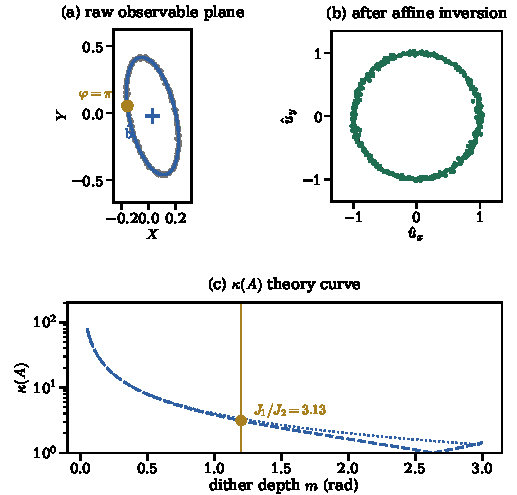
\includegraphics[width=\columnwidth]{figs/fig_affine_mzm.pdf}
\caption{仿射标定与导频深度设计。(a)(b)~标定示例（$m{=}1.2$、$\sigma{=}0.005$、$N{=}360$，含通道增益失配、$10^\circ$ 参考轴偏转、交叉耦合~$\varepsilon{=}0.10$ 与观测平移）：(a)~原始观测平面上的拟合椭圆、中心~$\hat\bv$ 与~$\varphi{=}\pi$ 基准点；(b)~回拉样本~$\hat\uv=B(\zv-\hat\bv)$ 落于单位圆。(c)~设计曲线：$J_1(m)$、$J_2(m)$（左轴）与条件数~$\kappa(A)$（理想链路下为~$J_1/J_2$，$m\gtrsim2.6$ 后两者互换）及其小~$m$ 渐近~$4/m$（右轴，对数）；竖线为仿真所用~$m{=}1.2$：理想比值~$J_1/J_2=3.13$，含失配的仿真真值矩阵~$\kappa(A)=2.59$。}
\label{fig:affine}
\end{figure}

\begin{figure}[!t]
\centering
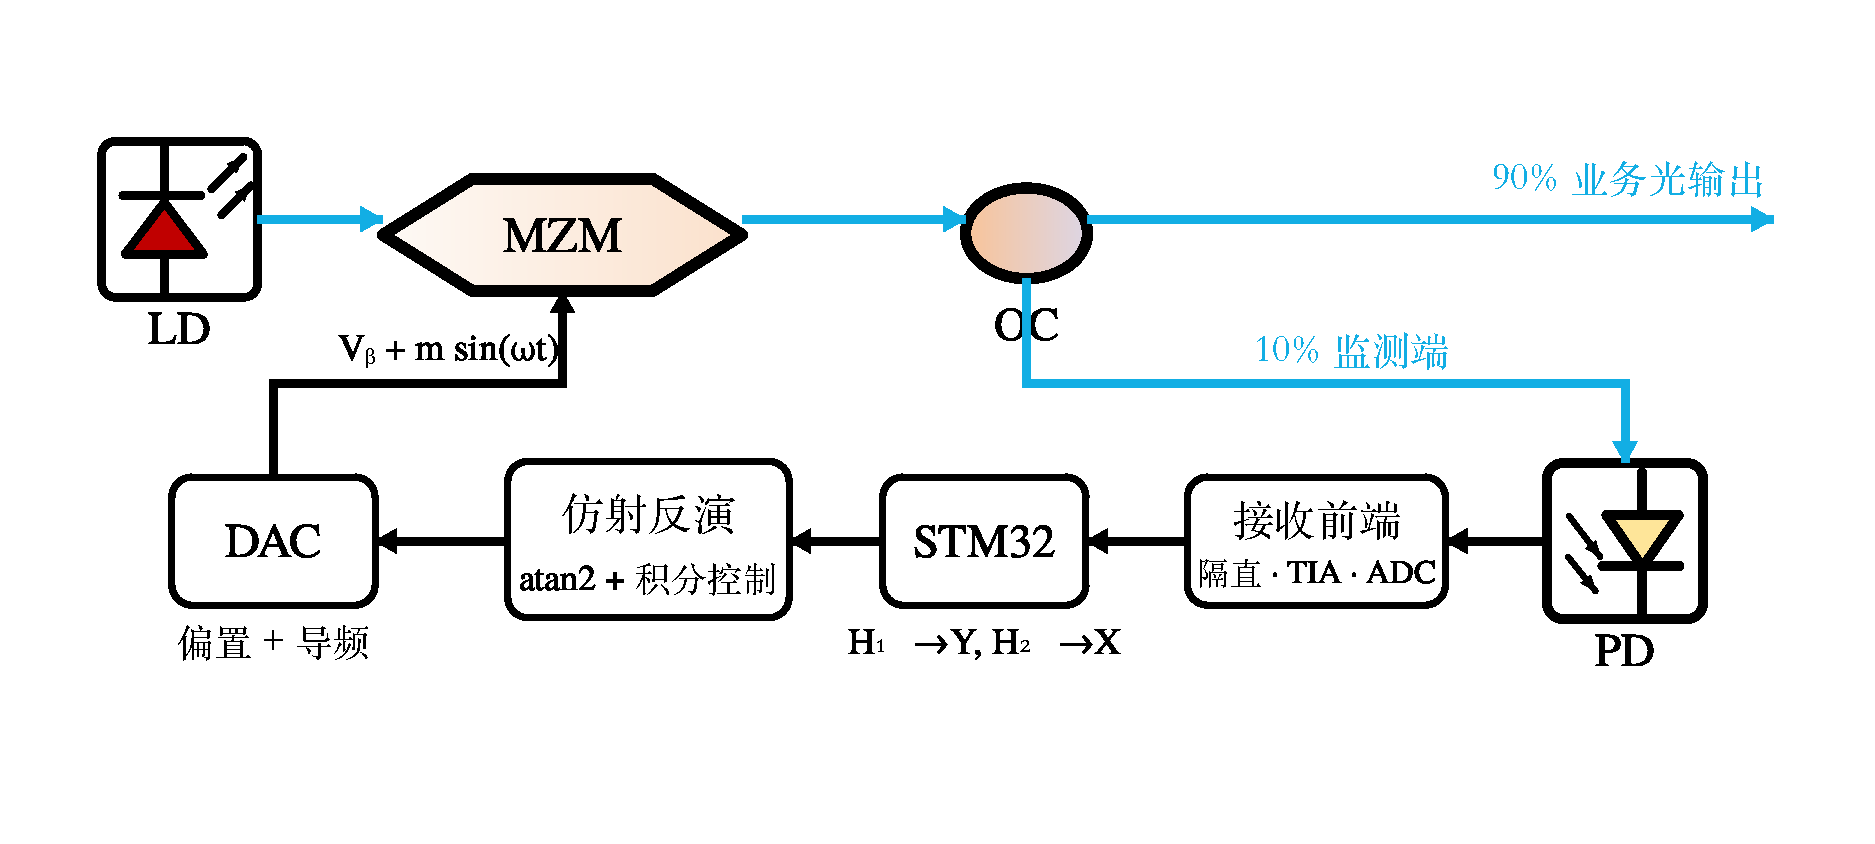
\includegraphics[width=\columnwidth]{figs/fig_arch_mzm_drawio.pdf}
\caption{单~MZM 任意点偏压闭环。光学抽头经光电探测器（PD）、隔直/跨阻放大器（TIA）和模数转换器（ADC）形成接收链；~STM32 以~Goertzel 提取~H1/H2，仿射逆与~$\atan$ 给出偏置相位，积分控制经数模转换器（DAC）叠加导频后回写~MZM。}
\label{fig:arch}
\end{figure}

\subsection{一致增益闭环}
闭环架构如图~\ref{fig:arch} 所示。取~$e=\operatorname{wrap}_{(-\pi,\pi]}(\hat\varphi_b-\varphi^\ast)$。当仿射模型成立时，解调后的相位误差与真实偏差直接对应，并与目标点位置解耦。配合常数执行斜率~$\partial\varphi_b/\partial V_b=\pi/V_\pi$，同一组控制参数可用于整个偏置周期。与依赖单坐标过零、幅值匹配或谐波比值的传统读出不同，仿射反演在~$A$ 满秩且规范已固定时覆盖全周期，并使闭环小信号增益不随目标相位变化。在已标定模型内，这对应消除标量读出的死区、分支歧义和标称增益偏差；噪声、有限带宽、执行器饱和与模型漂移仍进入实际误差预算。传统方案的静差由式~\eqref{eq:staticQ}--\eqref{eq:staticAM} 给出。本文采用增量积分更新；偏置漂移表现为低频扰动，其残余跟踪误差由环路带宽与漂移速率之比决定。

理想无附加时延、局部模型精确且执行器未饱和时，更新
$V_{k+1}=V_k-G e_k/(\pi/V_\pi)$ 给出
$e_{k+1}=(1-G)e_k$，故局部渐近稳定要求~$0<G<2$，单调收敛要求~$0<G\leq1$。若观测和执行间存在~$d$ 个额外控制周期的时延，则
$e_{k+1}=e_k-G e_{k-d}$，特征多项式为
$\lambda^{d+1}-\lambda^d+G=0$，允许增益区间随~$d$ 增大而收缩。实际有效增益还乘以执行斜率误差和局部解调斜率
$G_{\rm eff}=G(s/\hat s)(\partial\hat\varphi/\partial\varphi)$。
上电标定后，以独立预检测量局部斜率和尾段动态，并由原始误差序列的标准差、相邻控制周期交替幅度（周期--2 幅度）、饱和状态和最终绝对误差共同选择~$G$；尾段命令均值用于评价静态设定点映射，逐周期序列用于评价动态稳定性。

\begin{algorithm}[!t]
\caption{自标定与任意点闭环（残差监控与重定标层见第~\ref{sec:algo} 节算法~\ref{alg:cal}--\ref{alg:run}）}
\label{alg:mzm}
\begin{algorithmic}[1]
\Require 目标相位~$\varphi^\ast$、环路增益~$G$、样本数~$N$
\Ensure 解调算子~$(B,\hat\bv)$ 与逐周期偏压更新
\Statex \emph{\quad 标定阶段（上电执行一次）}
\State 慢扫偏压覆盖~$[0,2\pi)$，记录~$\{\zv_i,\bar\imath_i\}_{i=1}^N$
\State 中心化/归一后代数最小二乘拟合锥曲线~$\Rightarrow$ 中心~$\hat\bv$ 与~$M{=}(AA^{\T})^{-1}\succ0$
\State $B_0\gets M^{1/2}$；由轨道环绕方向定反射~$F\in\{I,\operatorname{diag}(1,-1)\}$
\State $\chi_i\gets\atan\!\bigl(FB_0(\zv_i-\hat\bv)\bigr)$；直流序列对~$(1,\cos\chi_i,\sin\chi_i)$ 回归得相位原点~$\hat\varphi_c$
\State $B\gets R(-\hat\varphi_c)\,F\,B_0$；以回拉径向残差与直流规范回归残差自检（优先使用留出点），不通过则重扫
\Statex \emph{\quad 运行阶段（每控制周期）}
\State 读锁相输出~$\zv=(X,Y)^{\T}$（H2、H1，与式~\eqref{eq:entries} 同序）
\State $\hat\uv\gets B(\zv-\hat\bv)$；\quad $\hat\varphi_b\gets\atan(\hat u_y,\hat u_x)$
\State $e\gets\operatorname{wrap}_{(-\pi,\pi]}(\hat\varphi_b-\varphi^\ast)$
\State 积分更新~$V_b\gets V_b-G\,e\,V_\pi/\pi$ 写入偏压~DAC
\State 残差~$\rho\gets\bigl|\,\|\hat\uv\|-1\bigr|$；持续越限则触发重定标（算法~\ref{alg:cal}）
\end{algorithmic}
\end{algorithm}

\section{噪声与导频深度设计}
\label{sec:noise}
本节回答导频深度~$m$ 的选取问题。绝对相位噪声由~$A$ 相对观测噪声协方差的尺度决定，条件数~$\kappa(A)$ 只描述最坏与最好方向之间的各向异性。记观测噪声协方差为~$\Sigma_n$，沿切向~$\tv(\varphi)=(-\sin\varphi,\cos\varphi)^{\T}$ 对~\eqref{eq:affine} 作一阶摄动，相位估计方差为
\begin{equation}
\begin{aligned}
\sigma^2_{\hat\varphi}(\varphi)
&=\tv^{\T}A^{-1}\Sigma_nA^{-\T}\tv\\
&\xrightarrow{\Sigma_n=\sigma^2I}\sigma^2\,\tv^{\T}(A^{\T}A)^{-1}\tv
\le\frac{\sigma^2}{\sigma^2_{\min}(A)}.
\end{aligned}
\label{eq:var}
\end{equation}
其几何含义如下。偏置相位只沿椭圆切向移动，观测噪声先投影到该方向，再经~$A^{-1}$ 拉回相位域。因此\emph{相位噪声等于测量噪声~$\sigma$ 除以椭圆在该方向上的拉伸量}：椭圆越扁，被压短方向上的相位噪声越大，最坏情形由最小奇异值~$\sigma_{\min}(A)$ 封顶。

条件数~$\kappa(A)=\sqrt{\lambda_{\max}(M)/\lambda_{\min}(M)}$ 是椭圆长短轴之比。理想链路下~$A=\operatorname{diag}(\eta\kappa_2,-\eta\kappa_1)$，故在~$J_1>J_2>0$ 的区间内~$\kappa(A)=J_1(m)/J_2(m)$；小~$m$ 时~$J_1\approx m/2$、$J_2\approx m^2/8$，所以~$\kappa(A)\sim4/m$。由较小奇异值对应的方向称为弱观测方向，其\emph{绝对}噪声增益为~$1/\sigma_{\min}(A)\propto1/J_2(m)\sim8/m^2$（固定接收增益与观测噪声时）。它与条件数不能互换：整体缩放~$A$ 不改变~$\kappa(A)$，却会改变式~\eqref{eq:var} 的相位方差。图~\ref{fig:affine}(c) 因而给出两个互补读数：$J_1,J_2$ 决定绝对观测灵敏度，$\kappa(A)$ 决定方向间不均匀性。$m$ 过小时~H2 被噪声淹没；$m$ 过大时导频损伤随~$m^2$ 增大并激起更高次谐波。本文仿真取~$m{=}1.2$，是兼顾这两项约束的一个示例工作点。实际设计应在导频扰动预算内最小化最坏相位方差~$\max_\varphi\tv^{\T}A^{-1}\Sigma_nA^{-\T}\tv$，最优~$m$ 随具体链路而变。

在模型正确、标定样本数与每点平均长度共同趋于无穷时，将标定参数直接代入式~\eqref{eq:demod} 的解调器（插入式估计）具有一致性，但不一定达到最小方差。Fisher 信息为~$\sigma^{-2}\|A\tv\|^2$，按马氏度量向椭圆投影可达~Cram\'er--Rao 界；当~$\kappa(A)$ 适中时，二者差异为二阶。在特殊点处，该框架复现与传统方法相同的噪声地板~$\sigma_Y/(\eta\kappa_1)$ 与~$\sigma_X/(\eta\kappa_2)$；其作用是让特殊点之外的相位同样获得有界的解调噪声。

\section{基于仿射模型的偏压控制算法设计}
\label{sec:algo}
前述理论可组织成一个两阶段控制流程（图~\ref{fig:flow}）。标定阶段执行偏压扫描、模型辨识、规范固定和残差自检；运行阶段在每个控制周期读取锁相输出，完成相位解调、误差计算和积分更新，并用圆残差监测椭圆中心、尺度或形状的变化。圆残差采用指数加权移动平均（exponentially weighted moving average, EWMA）滤波；若其持续越限~$N_{\rm p}$ 个周期，则触发具有充分激励的重定标扫描。算法~\ref{alg:cal} 与算法~\ref{alg:run} 分别给出两阶段伪代码；二者在第~\ref{sec:calib} 节算法~\ref{alg:mzm} 的流程之上加入残差监控。

\begin{figure}[!t]
\centering
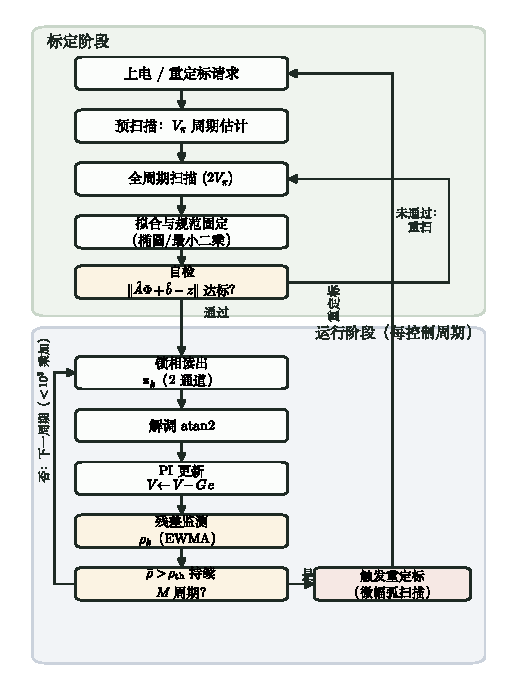
\includegraphics[width=\columnwidth]{figs/fig_flow_mzm.pdf}
\caption{监控状态机：上为标定阶段（扫描$\to$辨识与规范固定$\to$自检），下为运行阶段的每周期回路（锁相读出$\to$解调$\to$积分更新$\to$残差监测）。残差越限持续~$N_{\rm p}$ 周期后返回标定通道；本文实测采用全周期重扫。}
\label{fig:flow}
\end{figure}

\begin{algorithm}[!t]
\caption{自标定与规范固定（上电或重定标触发时执行）}
\label{alg:cal}
\begin{algorithmic}[1]
\Require 样本数~$N$；通道集~$K{=}2$
\Ensure 解调参数~$B,\hat\bv$ 与残差阈值~$\rho_{\rm th}$
\State 预扫描估计~$V_\pi$（基波周期）
\State 全周期扫描记录~$\{\zv_k,\bar\imath_k\}_{k=1}^N$
\State 中心化/归一后代数最小二乘拟合锥曲线~$\Rightarrow$ 中心~$\hat\bv$ 与~$M\succ0$；$B_0\gets M^{1/2}$
\State 由轨道环绕方向定反射~$F$；$\chi_k\gets\atan\!\bigl(FB_0(\zv_k-\hat\bv)\bigr)$
\State 直流序列对~$(1,\cos\chi_k,\sin\chi_k)$ 回归得~$\hat\varphi_c$；$B\gets R(-\hat\varphi_c)FB_0$
\State 自检：$\rho_k{=}\bigl|\|B(\zv_k-\hat\bv)\|-1\bigr|$ 与直流规范回归残差的第~95 百分位数（P95）均低于标定阈值；不通过则重新扫描
\State 记录残差统计~$(\mu_\rho,\sigma_\rho)$，置~$\rho_{\rm th}=\mu_\rho+k_\sigma\sigma_\rho$（$k_\sigma\approx4$--$6$）
\end{algorithmic}
\end{algorithm}

\begin{algorithm}[!t]
\caption{运行时控制周期（含残差监测与重定标触发）}
\label{alg:run}
\begin{algorithmic}[1]
\Require 目标~$\varphi^\ast$、环路增益~$G$、阈值对~$(\rho_{\rm th},N_{\rm p})$
\State 读取锁相输出~$\zv_k$
\State $\hat\uv\gets B(\zv_k-\hat\bv)$；\quad $\hat\varphi_b\gets\atan(\hat u_y,\hat u_x)$；\quad $\rho_k\gets\bigl|\,\|\hat\uv\|-1\bigr|$
\State $e\gets\operatorname{wrap}(\hat\varphi_b-\varphi^\ast)$；\quad 积分更新~$V_b\gets V_b-G\,e\cdot V_\pi/\pi$ 写入偏压~DAC
\State 残差~EWMA：$\bar\rho\gets(1-\lambda)\bar\rho+\lambda\rho_k$
\If{$\bar\rho>\rho_{\rm th}$ 连续~$N_{\rm p}$ 周期}
  \State 暂停闭环，执行满足满秩激励的重定标扫描（调用算法~\ref{alg:cal}）
\EndIf
\Ensure 进入下一周期；全周期代价远低于~$10^3$ 次乘加
\end{algorithmic}
\end{algorithm}

实现时有三类参数需要整定。\emph{阈值整定}：$\rho_{\rm th}$ 由稳定标定末尾的残差分布给出，EWMA 与连续~$N_{\rm p}$ 周期判决在误触发率和检测延迟之间折中；独立重复事件用于估计统计误报率与检出率。\emph{重定标激励}：完整椭圆与规范重新辨识要求覆盖充分相位范围。台架采用~121 点全周期扫描；继承旧模型并施加正则约束后，局部微弧可更新局部参数，本文在仿真中检验了~$\pm0.3$~rad 的受限更新。\emph{残差可观测性}：圆残差~$\rho=|\|B(\zv-\hat\bv)\|-1|$ 对径向、中心和椭圆形状变化敏感。规范旋转~$A\mapsto AR$（$R\in O(2)$）保持椭圆集合不变，其相位偏移由直流相位锚点残差、周期参考点或受控激励监测。$\atan$ 可由坐标旋转数字计算（coordinate rotation digital computer, CORDIC）或查表实现，参数存储量为六个标量。

\section{数值验证}
\label{sec:numerics}

\subsection{仿真设置与主要结果}
数值验证直接按
$X=b_X+g_XJ_2(m)\cos\varphi_b+\varepsilon J_1(m)\sin\varphi_b+n_X$、
$Y=b_Y-g_YJ_1(m)\sin(\varphi_b+\delta)+n_Y$ 生成观测。因此，$g_X,g_Y$ 是相对通道增益，$\delta$ 是~H1 参考轴偏转角，$\varepsilon$ 是~H2 对~H1 坐标的交叉耦合系数，与第~\ref{sec:affine} 节的导频二次谐波系数~$\varepsilon_h$ 不同；$b_X,b_Y$ 是观测平移，$n_X,n_Y$ 是标准差~$\sigma$ 的独立高斯噪声。仿真参数为~$m{=}1.2$、$g_X{=}1.18$、$g_Y{=}0.88$、$\delta{=}10^\circ$、$\varepsilon{=}0.10$、$\bv=(0.030,-0.022)^{\T}$、$\sigma{=}0.005$、$N{=}360$。闭环比较还向所有控制器施加同一条随机游走加慢正弦漂移序列，以隔离解调结构的差异。该组失配强于当前台架，用于构造受控的混合应力场景。主要结果汇总于表~\ref{tab:results}。

\begin{table}[!t]
\caption{数值验证结果。误差均为偏置相位误差。}
\label{tab:results}
\centering
\footnotesize
\setlength{\tabcolsep}{2.8pt}
\renewcommand{\arraystretch}{1.05}
\begin{tabular}{@{}p{0.38\columnwidth}p{0.25\columnwidth}p{0.29\columnwidth}@{}}
\toprule
验证项 & 结果 & 设置\\
\midrule
\multicolumn{3}{@{}l}{\emph{模型闭合与标定}}\\[1pt]
全周期零噪声解调 & $0.0000$~mrad & 数值精度\\
$\hat A$ 对真值~$A$ & $0.00\%$ & Frobenius 误差\\
含噪标定（中位／P95） & $2.35/6.25$~mrad & $\sigma{=}0.005$\\
直流回归／argmin & ${\sim}2/{\sim}42$~mrad & $N{=}360$\\
$\kappa(A)$（受扰／理想） & $2.59/3.13$ & $m{=}1.2$\\
\addlinespace[2pt]
\multicolumn{3}{@{}l}{\emph{闭环与监控动态}}\\[1pt]
仿射／H1 幅值匹配~RMS & $12.7/1315$~mrad & $\varphi^\ast{=}1.9$\\
捕获时间常数 & $5.6$ 周期 & $1/G$；四目标\\
阶跃整定时间 & $20$--$22$ 周期 & $20$~mrad 误差带\\
重定标判决延迟 & $31$ 周期 & 圆残差~EWMA\\
重定标后~RMS & $13.7$~mrad & 突变前~$12.6$~mrad\\
\bottomrule
\end{tabular}
\end{table}

零噪声实验首先检验模型闭合性。全周期最大解调误差为~$0.0000$~mrad（数值精度），$\hat A$ 相对真值的~Frobenius 误差~$0.00\%$，表明式~\eqref{eq:affine} 在仿真模型内是精确结构而非小信号近似。受扰真值的条件数为~$2.59$（理想比值~$3.13$），给出后续噪声分析所用的方向各向异性。

含噪标定实验考察规范固定和模型反演的稳定性。在~$\sigma{=}0.005$ 时，解调偏差中位~$2.35$~mrad，P95~$6.25$~mrad。图~\ref{fig:gauge} 给出直流回归规范与直流极小值~argmin 基准的对比：两种规范的中位偏差为~${\sim}2$ 对~${\sim}42$~mrad；前者随~$N^{-1/2}$ 收缩，后者受平坦极小值影响而几乎不收缩。

在任意目标点~$\varphi^\ast=1.9$ 处，闭环~RMS 为仿射~$12.7$~mrad、H1 幅值匹配~$1315$~mrad，后者的静差主要来自未辨识的仿射失配。图~\ref{fig:sweep} 将比较扩展到目标相位网格，并加入等信息对角二维基线：该基线与完整仿射方法使用相同观测通道、真值观测平移和对角增益，只将~$A$ 的非对角项置零。其残余相位偏差说明，二维观测提供全周期坐标，完整仿射校正进一步辨识非正交通道。统一仿真模型隔离非对角校正的贡献，硬件扫描则检验真实链路中的模型拟合。

\begin{figure}[!t]
\centering
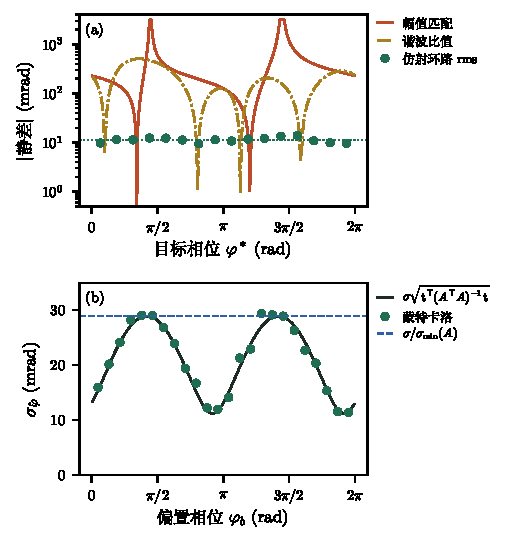
\includegraphics[width=\columnwidth]{figs/fig_sweep_mzm.pdf}
\caption{任意点性能随目标相位的分布。(a)~H1 幅值匹配、谐波比值、等信息对角二维~$\atan$ 与完整仿射环路。对角二维基线已使用真值观测平移和对角增益，但忽略~$A$ 的非对角项；圆点为含同一漂移序列与噪声的仿射闭环~RMS。(b)~式~\eqref{eq:var} 的理论噪声、蒙特卡洛结果与上界~$\sigma/\sigma_{\min}(A)$。}
\label{fig:sweep}
\end{figure}

\begin{figure}[!t]
\centering
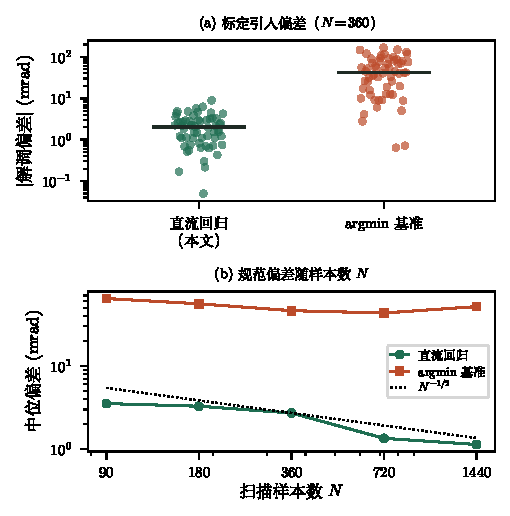
\includegraphics[width=\columnwidth]{figs/fig_gauge_mzm.pdf}
\caption{规范固定方案对照。(a)~$N{=}360$ 时标定引入的解调偏差分布：直流回归规范对~argmin 基准（横杠为中位数）；(b)~偏差中位数随扫描样本数~$N$ 的标度：回归规范按~$N^{-1/2}$ 收缩，argmin 基准受平坦极小值限制几乎不收缩。}
\label{fig:gauge}
\end{figure}

\subsection{算法级行为验证}
图~\ref{fig:acqstep} 验证算法~\ref{alg:cal}--\ref{alg:run} 的目标点无关动态。图~\ref{fig:acqstep}(a) 给出捕获瞬态：从~$1.5$~rad 的初始偏差出发，不同目标点的误差衰减曲线基本重合，与理论包络~$(1-G)^n$ 一致，对应时间常数~$1/G\approx5.6$ 个周期。

图~\ref{fig:acqstep}(b) 给出设定点阶跃结果：目标在五个任意相位间切换，各步进入~$20$~mrad 误差带的整定时间为~$20$--$22$ 个周期，与目标点无关。

残差触发路径采用受控漂移突变检验。在第~$1200$ 周期令~$g_X{:}\,1.18\!\to\!0.85$ 并改变~$b_x$ 后，圆残差~EWMA 越过阈值~$\rho_{\rm th}{=}0.06$，经~$31$ 个周期判决延迟触发重定标。失配期锁定误差升至~$275$~mrad（RMS），重定标后恢复至~$13.7$~mrad（突变前~$12.6$），对应结果汇总于表~\ref{tab:results}。

\begin{figure}[!t]
\centering
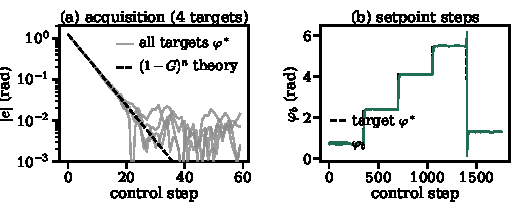
\includegraphics[width=\columnwidth]{figs/fig_acqstep_mzm.pdf}
\caption{捕获瞬态与设定点阶跃。(a)~捕获与一致增益验证：四个任意目标点（自~$1.5$~rad 偏差捕获）的误差曲线相互重合并贴合理论包络~$(1-G)^n$。(b)~设定点阶跃序列：目标在五个任意相位间阶跃，各步整定~$20$--$22$ 周期（至~$20$~mrad）且逐步一致。}
\label{fig:acqstep}
\end{figure}

\section{实验验证}
\label{sec:exp}
本节用四组实验检验二维仿射观测：全周期标定回答模型能否由实测谐波辨识；16 点扫描比较二维反演与~H1 幅值匹配基线；长记录刻画闭环动态；RF 加载和静态重复实验分别检验逐状态重新标定与采集参考的一致性。表~\ref{tab:exp} 汇总各组结果。

\subsection{实验平台与评价协议}
实验平台如图~\ref{fig:exp_mzm} 所示。$1550$~nm、约~$9$~dBm 的分布反馈（distributed-feedback, DFB）激光器驱动被测~MZM，输出经~1:9 光耦分为交流导频监测链与~RF 测量链。$10\%$ 光口接入自研偏压控制板内的~PD、隔直/TIA 和~ADC；STM32H523 以~$64$~kSPS 采样，并用~20~ms Goertzel 块提取~1/2~kHz 的~H1/H2，DAC8568 将上位机计算的偏置与导频回写至调制器。本次实验以~DM858E 数字万用表采集~PD 直流输出，生成全周期电压--相位标签并执行静态评价。50~MHz 加载时，DG922 Pro 驱动射频口，$90\%$ 光口经~PP-10G 接收机送入~FSV30。

\begin{figure*}[!t]
\centering
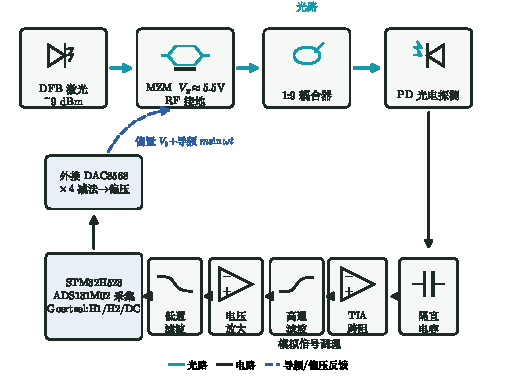
\includegraphics[width=\textwidth]{figs/fig_exp_mzm.pdf}
\caption{实测平台与信号流。自研偏压控制板集成~PD、隔直/TIA、ADC、偏压控制器和多通道~DAC；控制器通过通用串行总线（USB）串口与个人计算机（PC）上位机交换谐波与偏置命令，PC 完成仿射反演和积分更新。独立直流观测支路生成相位标签并评价静态目标；50~MHz RF 加载支路用于检验逐状态重新标定。灰色点线表示仪器控制与数据记录。}
\label{fig:exp_mzm}
\end{figure*}

实验中，$A_p$ 表示施加在偏压线上的导频电压幅值，对应理论模型中的~$V_d$，因此~$m=\pi A_p/V_\pi$。开环双向慢扫生成~$V_\pi$、$\varphi_0$ 和主闭环采用的相位标签回归标定；同批~H1/H2 数据还用于独立回放第~\ref{sec:calib} 节的椭圆--直流规范方法，以检验不直接使用逐点相位标签时的模型辨识与规范固定。五折交错留出按采样序号模~5 分组，每次用其中四组重新拟合直流标尺和标定参数，并仅在未参与拟合的一组上计算相位误差，最后汇总五组留出误差。

16 个目标点的静态响应采用两种电压--相位标尺评价：各目标附近的直流局部线性标尺，以及全周期宽扫映射。每个目标取控制记录后~40\% 的偏压命令均值，将该均值重新写入调制器并采集直流观测，再由局部标尺生成静态相位标签；由此得到的跨目标静态~RMS 与逐控制周期的时间~RMS 分别描述设定点映射和动态波动。RF 实验在每个功率态重新标定后测试~8 个目标；静态重复实验在~5 个全周期偏置点比较无重启、发生器重启、采集器重启和联合重启四种条件，每种条件重复~12 次。H1 幅值匹配基线与本文方法共用采集链和执行器，仅将二维相位反演换成~H1 单坐标读出。

\begin{table}[!t]
\caption{硬件验证结果。各任务按所列协议独立评价。}
\label{tab:exp}
\centering
\footnotesize
\setlength{\tabcolsep}{2.4pt}
\renewcommand{\arraystretch}{1.08}
\begin{tabular}{@{}
  >{\raggedright\arraybackslash}p{0.36\columnwidth}
  >{\raggedright\arraybackslash}p{0.33\columnwidth}
  >{\raggedleft\arraybackslash}p{0.23\columnwidth}@{}}
\toprule
验证任务 & 协议 & 实验结果\\
\midrule
\multicolumn{3}{@{}l}{\emph{标定与静态映射}}\\
相位标签回归误差 & $A_p{=}0.15$~V；拟合内 & 中位~$27.3$~mrad\\
16 点跨目标~RMS：仿射 & 局部相位标尺 & $246$~mrad\\
16 点跨目标~RMS：H1 幅值匹配 & 同上 & $1241$~mrad\\
观测各向异性~$\kappa(A)$ & $m{=}0.092$ & $45.24$\\
\addlinespace[1pt]
\multicolumn{3}{@{}l}{\emph{闭环动态}}\\
漂移检测延迟 & 残差触发 & $6$ 周期\\
重定标后时间~RMS & 121 点重扫 & $396$~mrad\\
3~h 重定标事件 & 连续记录 & 0 次\\
3~h 稀疏相位评价~RMS & 60 点 & $487$~mrad\\
\addlinespace[1pt]
\multicolumn{3}{@{}l}{\emph{RF 状态与采集重复性}}\\
RF 开启跨目标~RMS：最大 & $0$--$13$~dBm；逐态重新标定 & $192.5$~mrad\\
RF 关闭跨目标~RMS & 参考状态 & $166.1$~mrad\\
静态~H1 圆标准差：最大 & 5 点$\times$4 态$\times$12 次 & $0.330$~mrad\\
\bottomrule
\end{tabular}
\end{table}

\subsection{仿射模型标定与样本外相位反演}

\begin{figure}[!t]
\centering
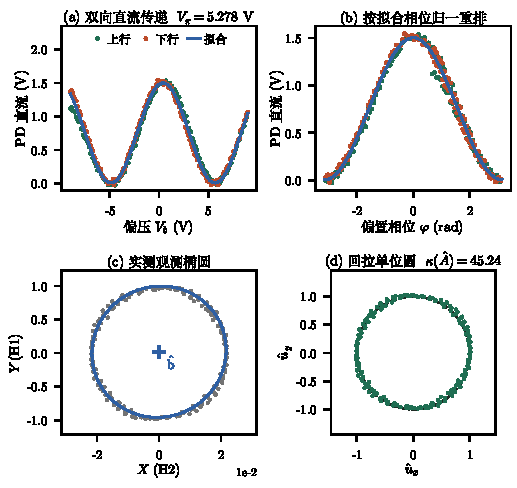
\includegraphics[width=\columnwidth]{figs/fig_expcal_mzm.pdf}
\caption{直流标尺、仿射标定与独立规范回放。(a) 直流双向慢扫及余弦拟合，上/下行~$V_\pi=5.36/5.20$~V，平均~$5.28$~V；(b) $A_p=0.15$~V（$m=0.092$）时的~H2/H1 观测轨迹，横纵轴分别按数据范围缩放，刻度保留各自真实尺度；$\kappa(\hat A)=45.24$ 表明~H2 方向为弱观测方向；(c) 主闭环采用的相位标签回归估计~$(A,\bv)$，并将拟合样本回拉至单位圆，拟合内中位误差为~$27.3$~mrad。独立的椭圆--直流规范回放中位误差与第~95 百分位数（P95）分别为~49.2 和~115.3~mrad。}
\label{fig:expcal}
\end{figure}

直流双向传递曲线给出上、下行~$V_\pi=5.36/5.20$~V，平均~$5.28$~V（图~\ref{fig:expcal}(a)）。以该标尺生成相位标签后，主闭环采用的相位标签回归把观测椭圆回拉至单位圆，拟合内中位误差为~27.3~mrad；同批数据上的椭圆--直流规范回放不直接使用逐点相位标签，得到中位~49.2~mrad 和~P95~115.3~mrad（图~\ref{fig:expcal}(b)(c)）。后者用于独立检验模型辨识与规范固定，不构成另一套控制律。

五折交错留出的中位/P95/RMS 为：相位标签回归路径~27.7/105.6/53.7~mrad，椭圆--直流规范路径~48.7/114.1/61.7~mrad。将~$A$ 的非对角项置零后，完整二维与等信息对角二维基线的留出~RMS 分别为~53.7 和~60.3~mrad；该基线保留同一训练数据估计的观测平移与两轴增益，只去除非对角混合。实测非对角项的~Frobenius 范数占比为~0.85\%，与该台架接近对角的观测链一致。

\subsection{全周期目标响应与闭环动态}

\begin{figure}[!t]
\centering
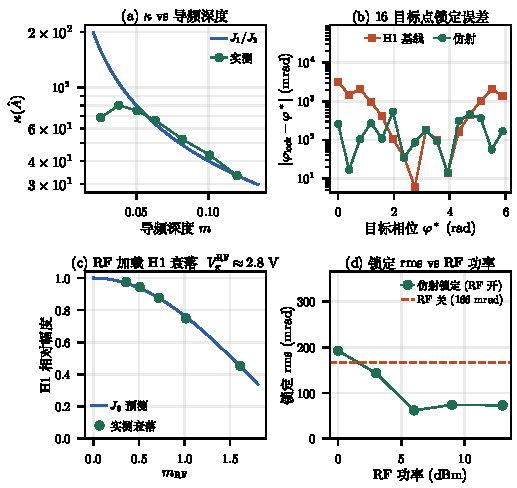
\includegraphics[width=\columnwidth]{figs/fig_expperf_mzm.pdf}
\caption{全周期目标响应与~RF 状态重新标定。(a) 椭圆条件数~$\kappa(\hat A)$ 随导频深度~$m$ 的趋势，$\kappa$ 刻画观测各向异性。(b) 16 个目标的静态评价：二维仿射反演和~H1 幅值匹配基线的跨目标~RMS 分别为~246 和~1241~mrad。(c) 50~MHz 单音下~H1 衰落及同一数据的~$J_0$ 拟合，等效~$V_\pi^{\rm RF}\approx2.8$~V；(d) 每个~RF 功率态重新标定后的~8 点跨目标~RMS 与~$\kappa(\hat A)$。}
\label{fig:expperf}
\end{figure}

导频深度~$m\approx0.09$--$0.12$ 时，实测~$\kappa(\hat A)\approx45$，H2 主导的弱观测方向决定最小奇异值和相位噪声增益（图~\ref{fig:expperf}(a)）。16 点扫描按上述后~40\% 命令均值回写，并由直流局部标尺生成静态相位标签；二维仿射反演的跨目标~RMS 为~246~mrad，H1 幅值匹配基线为~1241~mrad（图~\ref{fig:expperf}(b)）。全周期宽扫映射得到相同排序，对应~342 和~2491~mrad。局部相位标尺评价的响应斜率和~$R^2$ 为~1.052 和~0.986；全周期宽扫映射的对应值为~1.039 和~0.980。15 个相邻步进中~14 个方向一致，16 个点的绝对误差均小于~$\pi/4$，因而覆盖全周期。

\begin{figure}[!t]
\centering
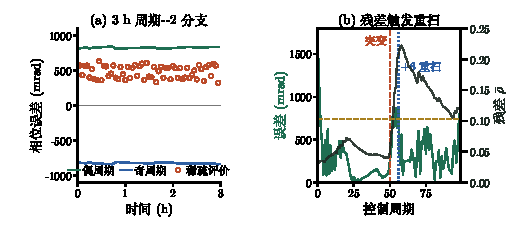
\includegraphics[width=\columnwidth]{figs/fig_expdiag_mzm.pdf}
\caption{闭环动态诊断。(a)~3~h 记录中奇偶控制周期相位误差的~61 点移动均值及稀疏相位评价，两个分支对应持续周期--2 极限环，逐周期~RMS 为~827~mrad、一阶滞后（lag-1）相关系数为~$-0.995$。(b)~导频幅度阶跃后，圆残差在~6 个控制周期内触发~121 点重扫，尾段时间~RMS 为~396~mrad。}
\label{fig:expdynrepeat}
\end{figure}

逐周期数据揭示了静态中心以外的闭环动态：6/16 个目标的尾段标准差为~0.716--1.067~rad，合并尾段解调时间~RMS 为~571~mrad。相邻控制周期在两个误差分支间交替的状态称为周期--2 极限环；3~h 记录中的逐周期误差~RMS 为~827~mrad，一阶滞后相关系数为~$-0.995$（图~\ref{fig:expdynrepeat}(a)）。导频幅度阶跃后，圆残差在~6 个控制周期内触发~121 点重扫，尾段时间~RMS 为~396~mrad（图~\ref{fig:expdynrepeat}(b)）。这些记录把当前台架的动态约束定位到弱观测方向噪声、控制增益与端到端时延的耦合。

\subsection{RF 状态重新标定与采集重复性}
50~MHz 单音从~RF 关扫至~$+13$~dBm，并在每个功率态重新标定后测试~8 个目标。记施加在射频口的正弦峰值电压为~$V_{\rm pk}$，射频调制深度为~$m_{\rm RF}=\pi V_{\rm pk}/V_\pi^{\rm RF}$；等效射频半波电压~$V_\pi^{\rm RF}$ 由~H1 衰落曲线的~$J_0(m_{\rm RF})$ 拟合得到，实验值约为~2.8~V。各状态的~$\kappa(\hat A)$ 约为~45，跨目标~RMS 为~62--193~mrad（图~\ref{fig:expperf}(c)(d)），其中表~\ref{tab:exp} 的~192.5~mrad 为~RF 开启各功率态中的最大值。静态~RF 载荷改变后，逐状态重新标定即可恢复全周期相位坐标。

静态重复实验包含~240 次重复和~480 个~16 块采集窗；每次重复均在采集前后各记录两次直流观测，全部记录通过完整性、原始输入余量、时间顺序和校验和回放检查，最大绝对输入为~0.672~V，低于~0.95~V 余量门限。圆标准差用于刻画相位样本在单位圆上的离散程度。四种条件下的~H1 圆标准差最大为~0.330~mrad，相对无重启条件的最大增量为~0.287~mrad；H2 的最大圆标准差为~29.9~mrad，低于预注册的~50~mrad 共变门限。发生器、采集器及联合重启均未在~5 个偏置点中的至少~3 点同时达到“增大至两倍且增加不少于~20~mrad”的异常条件，因此重启不是观测变化的来源。

\section{讨论}
\label{sec:discussion}
\emph{持续激励与检测盲区。}本文方法依赖对~$(A,\bv)$ 的辨识。闭环稳态下，偏置相位停在目标附近，新的观测样本不再充分激励参数空间。圆残差可检测中心、尺度和形状变化，但对~$A\mapsto AR$ 的规范旋转不敏感。部署时需联合监测直流相位锚点，或周期性访问参考点；局部递推更新还须施加继承旧模型的正则约束。

\emph{漂移时间尺度。}重定标速度由漂移速率与闭环带宽之比决定。LiNbO$_3$/InP 器件的热致漂移常在秒至分钟量级，电荷重分布与光折变效应可延伸至分钟至小时~\cite{salvestrini2011,chen2011}。本文统一以控制周期报告动态：仿真重定标延迟为~31 周期，台架阶跃检测为~6 周期；台架受串口通信和~Goertzel 平均限制，单周期约为秒量级。将相位反演与积分更新移入板载固件可直接缩短计算和通信路径，实际带宽由端到端时延及其稳定裕度确定。

\emph{硬件实现。}对已有~H1/H2 双谐波锁相固件，运行时主要增加一次~$2{\times}2$ 乘加和一次~$\atan$，可由~CORDIC 或查表实现。板载化的关键设计量是定点精度、端到端时延和全周期重扫占用时间，而非计算复杂度。

\emph{适用范围。}仿射结构适用于线性接收、线性解调且扫描期间参数近似不变的链路；光电探测/跨阻非线性、偏压相关吸收和直流规范漂移会形成模型外残差。单器件实验验证了相位标签回归闭环，并以椭圆--直流规范独立回放检验模型辨识与规范固定；静态重复实验确认采集参考稳定，逐周期记录则把台架动态约束定位到控制增益、端到端时延与~H2 主导的弱观测方向噪声之间的耦合。H1 幅值匹配基线隔离单坐标死区和分支歧义；DLA2C~\cite{hu2026dla2c} 以训练和迭代搜索换取免测~H2，本文保留~H2 并通过闭式反演实现显式通道校正。

\emph{推广方向。}椭圆--直流规范路径可直接扩展到无标签硬件闭环，等信息对角二维基线能够量化非对角校正收益，跨器件测试则检验参数缩放与外部有效性。该框架还可推广到嵌套或多电极调制器；在线设计可用式~\eqref{eq:var} 的最坏相位方差联合优化导频深度与频率，并以相位锚点创新量补足圆残差的规范盲区。

\section{结论}
本文建立了线性接收--解调链下二维谐波观测的精确仿射结构，并将全周期相位可辨识性归结为两个条件：$A$ 满秩，以及绝对相位的~$O(2)$ 规范得到唯一固定。由此形成的模型辨识、规范固定和闭式~$\atan$ 反演，把任意点偏压控制写成一次标定后的相位反馈问题。数值实验验证了精确闭合、全周期反演和目标点无关的闭环增益；真实硬件在~16 个全周期目标点取得~246~mrad 的跨目标静态相位~RMS，H1 幅值匹配基线为~1241~mrad。样本外回放、静态重复和逐~RF 状态重新标定进一步验证了标定泛化、采集重复性与静态载荷下的可重标定性。逐周期实验识别出弱观测方向噪声、控制增益与端到端时延耦合形成的周期--2 极限环，为板载实现给出增益和稳定裕度约束。理论与测量共同说明，二维仿射观测为单~MZM 任意点偏压提供了可辨识、可标定且计算紧凑的控制坐标。

\begin{thebibliography}{30}

\bibitem{salvestrini2011}
J.~P. Salvestrini, L.~Guilbert, M.~Fontana, M.~Abarkan, and S.~Gille,
``Analysis and control of the {DC} drift in {LiNbO$_3$}-based
{Mach--Zehnder} modulators,'' \emph{J. Lightw. Technol.}, vol.~29,
no.~10, pp. 1522--1534, May 2011.

\bibitem{chen2011}
A.~Chen and E.~J. Murphy, Eds., \emph{Broadband Optical Modulators:
Science, Technology, and Applications}.\hskip 1em plus 0.5em minus
0.4em\relax Boca Raton, FL, USA: CRC Press, 2011.

\bibitem{wang2018}
C.~Wang, M.~Zhang, X.~Chen, M.~Bertrand, A.~Shams-Ansari, S.~Chandrasekhar,
P.~Winzer, and M.~Lon\v{c}ar, ``Integrated lithium niobate electro-optic
modulators operating at {CMOS}-compatible voltages,'' \emph{Nature},
vol. 562, pp. 101--104, Oct. 2018.

\bibitem{wang2022}
M.~Wang, J.~Li, H.~Yao, X.~Li, J.~Wu, K.~S. Chiang, and K.~Chen,
``Thin-film lithium-niobate modulator with a combined passive bias and
thermo-optic bias,'' \emph{Opt. Express}, vol.~30, no.~22,
pp. 39706--39715, Oct. 2022.

\bibitem{cho2006}
P.~S. Cho, J.~B. Khurgin, and I.~Shpantzer, ``Closed-loop bias control
of optical quadrature modulator,'' \emph{IEEE Photon. Technol. Lett.},
vol.~18, no.~21, pp. 2209--2211, Nov. 2006.

\bibitem{sotoodeh2011}
M.~Sotoodeh, Y.~Beaulieu, J.~Harley, and D.~L. McGhan, ``Modulator bias
and optical power control of optical complex {E}-field modulators,''
\emph{J. Lightw. Technol.}, vol.~29, no.~15, pp. 2235--2248, Aug. 2011.

\bibitem{kawakami2012}
H.~Kawakami, E.~Yoshida, and Y.~Miyamoto, ``Auto bias control technique
based on asymmetric bias dithering for optical {QPSK} modulation,''
\emph{J. Lightw. Technol.}, vol.~30, no.~7, pp. 962--968, Apr. 2012.

\bibitem{fu2013}
Y.~Fu, X.~Zhang, B.~Hraimel, T.~Liu, and D.~Shen, ``Mach--Zehnder: A review
of bias control techniques for {Mach--Zehnder} modulators in photonic
analog links,'' \emph{IEEE Microw. Mag.}, vol.~14, no.~7, pp. 102--107,
Nov. 2013.

\bibitem{li2017}
X.~Li, L.~Deng, X.~Chen, M.~Cheng, S.~Fu, M.~Tang, and D.~Liu,
``Modulation-format-free and automatic bias control for optical {IQ}
modulators based on dither-correlation detection,'' \emph{Opt. Express},
vol.~25, no.~8, p. 9333, Apr. 2017.

\bibitem{yao2009}
J.~Yao, ``Microwave photonics,'' \emph{J. Lightw. Technol.}, vol.~27,
no.~3, pp. 314--335, Feb. 2009.

\bibitem{capmany2007}
J.~Capmany and D.~Novak, ``Microwave photonics combines two worlds,''
\emph{Nat. Photon.}, vol.~1, no.~6, pp. 319--330, Jun. 2007.

\bibitem{izutsu1981}
M.~Izutsu, S.~Shikama, and T.~Sueta, ``Integrated optical {SSB}
modulator/frequency shifter,'' \emph{IEEE J. Quantum Electron.},
vol.~17, no.~11, pp. 2225--2227, Nov. 1981.

\bibitem{shen2017}
Y.~Shen, N.~C. Harris, S.~Skirlo, M.~Prabhu, T.~Baehr-Jones, M.~Hochberg,
X.~Sun, S.~Zhao, H.~Larochelle, D.~Englund, and M.~Solja\v{c}i\'c,
``Deep learning with coherent nanophotonic circuits,''
\emph{Nat. Photon.}, vol.~11, no.~7, pp. 441--446, Jul. 2017.

\bibitem{wang2010}
L.~L. Wang and T.~Kowalczyk, ``A versatile bias control technique for
any-point locking in lithium niobate {Mach--Zehnder} modulators,''
\emph{J. Lightw. Technol.}, vol.~28, no.~11, pp. 1703--1706, Jun. 2010.

\bibitem{tao2014}
J.-J. Tao, Y.-A. Zhang, J.-N. Zhang, X.-G. Yuan, Y.-Q. Huang, and Y.-P. Li,
``A novel auto-bias control scheme for stabilizing lithium niobate
{Mach--Zehnder} modulator at any operating point,''
\emph{Optoelectron. Lett.}, vol.~10, no.~1, pp. 21--23, Jan. 2014.

\bibitem{yuan2019}
X.~Yuan, Y.~Zhang, J.~Zhang, and M.~Zhang, ``Any point bias control
technique for {MZ} modulator,'' \emph{Optik}, vol. 178, pp. 918--922,
Feb. 2019.

\bibitem{li2018}
X.~Li, L.~Deng, X.~Chen, H.~Song, Y.~Liu, M.~Cheng, S.~Fu, M.~Tang,
M.~Zhang, and D.~Liu, ``Arbitrary bias point control technique for optical
{IQ} modulator based on dither-correlation detection,''
\emph{J. Lightw. Technol.}, vol.~36, no.~18, pp. 3824--3836, Sep. 2018.

\bibitem{teng2023}
J.~Teng \emph{et al.}, ``Arbitrary bias control of {LiNbO$_3$}-based
{Mach--Zehnder} intensity modulators for {QKD} system,''
\emph{EPJ Quantum Technol.}, vol.~10, Art.~no.~33, Sep. 2023.

\bibitem{weller2025}
S.~Weller, S.~Haxha, J.~Galdeano, and I.~McKenzie, ``Bias control for
{Mach--Zehnder} modulators: A gradient-based optimization approach,''
\emph{IEEE Trans. Microw. Theory Techn.}, vol.~73, no.~12,
pp. 10678--10690, Dec. 2025.

\bibitem{peng2025}
M.~Peng, S.~Yan, J.~Tang, Q.~Li, E.~Yan, J.~Huang, X.~Lei, L.~Zhu, and
G.~Wang, ``Ultralow-dither automatic bias control on {IQ} modulators for
optical single-sideband modulation via adaptive extended {Kalman}
filtering-enhanced correlation detection,'' \emph{Opt. Express},
vol.~33, no.~20, p. 43221, Oct. 2025.

\bibitem{hu2026dla2c}
X.~Hu, Y.~Dai, Y.~Li, S.~Chen, T.~Liu, Z.~Guo, Q.~Cai, J.~Yang,
T.~Zhou, Y.~Peng, and T.~Jiang, ``{DLA2C}: Deep-learning-based advanced
adaptive control for {Mach--Zehnder} modulators,'' \emph{Chin. Opt. Lett.},
vol.~24, no.~1, Art.~no.~011201, Jan. 2026,
doi: 10.3788/COL202624.011201.

\bibitem{heydemann1981}
P.~L.~M. Heydemann, ``Determination and correction of quadrature fringe
measurement errors in interferometers,'' \emph{Appl. Opt.}, vol.~20,
no.~19, pp. 3382--3384, 1981.

\bibitem{fitzgibbon1999}
A.~Fitzgibbon, M.~Pilu, and R.~B. Fisher, ``Direct least square fitting
of ellipses,'' \emph{IEEE Trans. Pattern Anal. Mach. Intell.}, vol.~21,
no.~5, pp. 476--480, May 1999.

\bibitem{svarny2022}
J.~Svarny and S.~Chladek, ``Model-based bias controller for a
{Mach--Zehnder} intensity modulator,'' \emph{J. Lightw. Technol.},
vol.~40, no.~3, pp. 720--727, Feb. 2022.

\end{thebibliography}

\end{document}
